\section{Results\label{sec:results}}
This section shows performance for the proposed bus charging algorithm and contains three subsections. Section \ref{sec:results:setup} describes the setup for the experiments. Section \ref{sec:results:prior} compares the proposed method with a previously published algorithm \cite{He_2019_Fast}. Section \ref{sec:results:time} discusses the difference in computation time between prior work and the current method.
\textcolor{red}{TODO: include blurb in the beginning that talks about how the current discrete method lacks precision with large step size and is computationally difficult with small ones.}
\subsection{Setup\label{sec:results:setup}}
\par The comparisons in this section consider a 5 bus 5 charger scenario with a charge rate of 300 kW. Each solution is expressed in terms of a MILP and solved up to a 2\% gap using Gurobi \cite{gurobi} unless otherwise specified. The uncontrolled loads from section \ref{sec:uncontrolled} are represented with a scaled version of historical data from the Trax Power SubStation at UTA. The scaling served to increase the difficulty of the charging problem and better illustrates the capabilities of our algorithm. 

\subsection{Cost Comparison with Prior Work\label{sec:results:prior}} 
This section compares the monthly cost of energy for the proposed method with two other methods. The first method is a baseline algorithm that simulates how bus drivers at the Utah Transit Authority (UTA) in Salt Lake City (SLC) charge by default. The second method comes from \cite{He_2019_Fast}, which was selected because it is very similar to the proposed algorithm. The charge plan for all three methods is computed using mixed integer linear programs as described below.  
\par Conversations with bus drivers at the UTA in SLC have shown that bus drivers generally top off their batteries whenever a charger is available. In essence, the bus drivers are solving a maximization problem by default as they maximise the number of charge sessions in a day. Hence, the baseline algorithm follows the constraints in equation \ref{eqn:objective:final} but incentivizes buses to charge as frequently as possible. Let $v_{\sigma}^{ijk}$ be the value of the objective function $v$ at the index corresponding to $\sigma_{ijk}$ from section \ref{sec:formulation:constraint}. By letting $v^{ijk}_{\sigma} = -1, \ \forall i,j,k$ and zero otherwise, the baseline method effectively maximizes the number of times a bus can charge.  
 All methods are evaluated according to the rate schedule in \cite{rocky_mountain_power_rocky_2021}. A comparison of all three algorithms is given in Fig. \ref{fig:costComparison}. Note how the cost of energy is generally the same for each algorithm and that the primary differences in cost come from come from the on-peak and facilities power charges, illustrating the need to minimize peak average power. To understand the difference in power management between the baseline and the proposed method, refer to Fig. \ref{fig:totalPower}. Note how the power for the proposed method (blue line) profile is almost completely flat, indicating a steady power use and is devoid of large power spikes. In comparison, the baseline algorithm (red line) is less steady and includes periods of significant power use, leading to the increased power charges in Fig. \ref{fig:costComparison}.
\par The proposed method improves upon \cite{He_2019_Fast} because it accounts for the effects of uncontrolled loads and costs of average power. The modest increase in the cost of energy from Fig. \ref{fig:costComparison} is significantly recouped by the savings in facilities power. The proposed method accomplishes this by charging more during on-peak periods to avoid charging when the uncontrolled loads are high, which can be seen in Fig.\ref{fig:powerPlot}. Note that from 8:00 to 4:00 the power from charging buses is complementary to the uncontrolled loads, resulting in a flat load profile whereas the load profile from \cite{He_2019_Fast} only minimizes charging during on-peak periods, resulting in the the reduced energy costs. 
\begin{figure}
	\centering
	\makeComparisonBarChartThree{media/7_objective/costComparison5Bus5ChargersAugmented.csv}{Cost (Dollars)}{Baseline}{He et al.}{Optimized}
	\caption{Cost comparison with prior work}
	\label{fig:costComparison}
\end{figure} 

\begin{figure*}
	\centering
	\makeComparisonTotalPower{media/7_objective/optimized5Bus5ChargerAugmentedTotalPowerPlot.csv}{media/7_objective/baseline5Bus5ChargerAugmentedTotalPowerPlot.csv}{15-Minute Average Power (kW)}{Optimized}{Baseline}
	\caption{15-Minute average power for one day}
	\label{fig:totalPower}
\end{figure*}
\begin{figure*}
	\centering
	\makeComparisonPower{media/7_objective/optimized5Bus5ChargerAugmentedPowerPlot.csv}{media/7_objective/HeEtAl5Bus5ChargerAugmentedPowerPlot.csv}{15-Minute Average Power (kW)}{Optimized}{He et al.}
	\caption{Comparison between uncontrolled and bus loads}
	\label{fig:powerPlot}
\end{figure*}

\subsection{Computation Time\label{sec:results:time}} 
As explained in the introduction, one motivation for this work was to extend the work by <mortensen> to include the benefits while avoiding the pitfalls of computation complexity. This section shows a comparison of work by \cite{mortensen_comprehensive_2021} which uses a network flow approach and discrete time axis to solve the charge problem. Because both the approach in \cite{mortensen_comprehensive_2021} and the approach in this paper include the full rate schedule, their monthly costs are comparable. However, because the approach from \cite{mortensen_comprehensive_2021} handles the time component discretely, higher fidelity time estimates become computationanlly prohibitive. 
\par Fig. \ref{fig:timeComparison} compares the computation time for the proposed algorithm with \cite{mortensen_comprehensive_2021} with a time step of one minute. The algorithms were run on a common desktop computer with 32 Gb of RAM and an 8 core 4 Gz processor and the method from \cite{mortensen_comprehensive_2021} was solved up to a 5\% gap. Note how the optimized algorithm is several orders of magnitude less to compute and gives the added benefit of floating point precision in its time estimates.
\begin{figure}
	\centering
	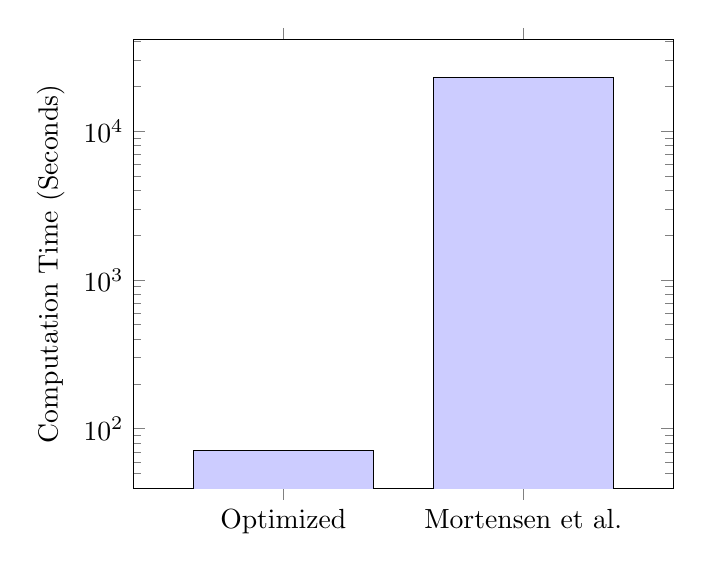
\begin{tikzpicture}
		\begin{axis}[ybar, ylabel=Computation Time (Seconds), ymode=log, xmin=0, xmax=1.8, xtick={0.5,1.3},xticklabels={Optimized, Mortensen et al.}]
			\addplot[fill=blue!20, bar width=0.6] coordinates{
			(0.5,71.187)
			(1.3,23013) 
		};
		\end{axis}
\end{tikzpicture}
	\caption{Comparison of computation time between the proposed algorithm and \cite{mortensen_comprehensive_2021}}
	\label{fig:timeComparison}
\end{figure}







